\documentclass[12pt]{article}

\usepackage{sbc-template}
\usepackage{graphicx}
\usepackage{hyperref}
\hypersetup{
    colorlinks,
    linkcolor=blue,
    citecolor=black,
    urlcolor=blue,
}
\usepackage[utf8]{inputenc}
\usepackage[brazil]{babel}
\usepackage[T1]{fontenc}
\usepackage[protrusion=true,expansion=true,final,babel]{microtype}
\usepackage{caption}
\usepackage{subcaption}
\usepackage{booktabs}

\renewcommand{\sectionautorefname}{Seção}
\renewcommand{\figureautorefname}{Figura}
\renewcommand{\tableautorefname}{Tabela}
     
\sloppy

\title{Acerca da melhora de um \textit{pipeline} de produção de pipoca}

\author{Giovanne César O. de Souza\inst{1}, Guilherme Eiji E. Hantani\inst{1},\\Eduardo Gil S. Cardoso\inst{1}, Igor Matheus S. Moreira\inst{1}}


\address{
    Faculdade de Computação -- Instituto de Ciências Exatas e Naturais\\
    Universidade Federal do Pará -- Rua Augusto Corrêa, 01 -- 66.075-110\\
    Belém -- Pará -- Brasil
    \email{\{giovanne.souza,guilherme.hantani\}@icen.ufpa.br}
    \vspace{-10pt}
    \email{\{eduardo.serrao.cardoso,igor.moreira\}@icen.ufpa.br}
}

\begin{document} 

\maketitle

\begin{abstract}
    In this deliverable for the Discrete Simulation discipline, a Kaggle data set that describes a popcorn production pipeline is exposed. A discrete simulation is created based on it, wherein scenarios are created in hopes of streamlining and accelerating the process. Two improvements in particular are analysed: maintain the heater always on and add a second pan to the system. The results indicate that both measures would result in a higher productivity; however, absent aspects in the simulation due to the lack of data must be considered.
\end{abstract}
     
\begin{resumo}
    Neste entregável para a disciplina Simulação Discreta, um conjunto de dados que descreve um \textit{pipeline} de produção de pipoca é exposto. Uma simulação discreta é criada baseada nele, em que cenários são criados na esperança de simplificar e acelerar o processo. Duas melhorias em particular são analisadas: manter o aquecedor sempre ligado e adicionar uma segunda panela ao sistema. Os resultados indicam que ambas as medidas resultariam em uma maior produtividade; todavia, aspectos ausentes na simulação devido à falta de dados hão de ser considerados.
\end{resumo}

\section{Introdução}

A simulação discreta pode ser definida como a modelagem da operação de um sistema fazendo uso de uma sequência de eventos discretos ao longo do tempo, da sorte que cada evento ocorre em um momento específico e promove uma mudança no estado do sistema \cite{robinson2014simulation}. Isto se mostra especialmente útil para fazer testes em modelos de sistema reais sem sujeitar o sistema real a qualquer estresse.

Sendo assim, a simulação discreta é comumente utilizada para a compreensão do funcionamento de um sistema, tal como o estudo do efeito de eventuais alterações em suas especificidades -- geralmente envolvendo gestão de recursos --, a fim de elaborar estratégias para atingir um objetivo (e.g., diminuição de custos, aumento de produtividade).

Neste artigo, analisaremos um sistema responsável por uma linha de produção de pipoca. Para isso, utilizaremos a linguagem de programação \texttt{python} e o módulo \texttt{simpy} para criar uma simulação discreta do processo. A partir dela, obteremos um \textit{baseline} de produtividade, com base no qual melhorias ao sistema serão propostas. Objetiva-se aqui maximizar a produtividade do processo produtivo.

As demais seções estão divididas como segue: a \autoref{sec:descricao_problema} contextualiza o problema e o conjunto de dados a ser analisado; a \autoref{sec:modelagem} descreve a modelagem feita a partir do conjunto de dados; a \autoref{sec:simulacao_resultados} expõe a simulação em si e os resultados dela advindos; a \autoref{sec:propostas} propõe melhorias ao processo produtivo sob análise; e a \autoref{sec:conclusao} finaliza este artigo com algumas considerações.

\section{Descrição do Problema}
\label{sec:descricao_problema}

Este trabalho fundamenta-se em um \textit{data set} obtido na plataforma \textit{Kaggle} (para acessá-lo, \href{https://www.kaggle.com/inIT-OWL/versatileproductionsystem}{clique aqui}), que descreve um sistema produtor de pipoca e é composto por vários arquivos \texttt{.csv}. Considerando o objetivo proposto, as análises contidas neste artigo foram realizadas sobre o arquivo \texttt{Production.csv}, composto por 7728 amostras e 16 atributos.

Cada amostra do arquivo em questão representa um registro do estado do sistema. Elas são compostas por quinze atributos do tipo \texttt{int} e um do tipo \texttt{float}. Um dos atributos contém \textit{Unix timestamps} documentando o momento de registro de cada amostra. Sete repetições completas do processo produtivo estão contidas neste arquivo.

O processo completo da produção consiste sucintamente no que segue: primeiramente, uma porção de milho é despejada em uma panela, e o aquecedor é ativado. Este aquece a panela e realiza o estouro do milho, causando a queda da pipoca em um copo. Uma vez cheio, o copo é despejado, resultando em uma porção de pipoca. Dada a disponibilidade de milho, o processo pode ser repetido indefinidamente.

Considerando que o arquivo \texttt{Production.csv} contém os estados das entidades relevantes e as amostras são coletadas com uma frequência razoável, pode-se retirar dele as entidades e os tempos de evento relevantes. As particularidades do pré-processamento e da modelagem de dados estão descritas na seção seguinte.

\section{Modelagem}
\label{sec:modelagem}

\begin{figure}[h]
    \centering
    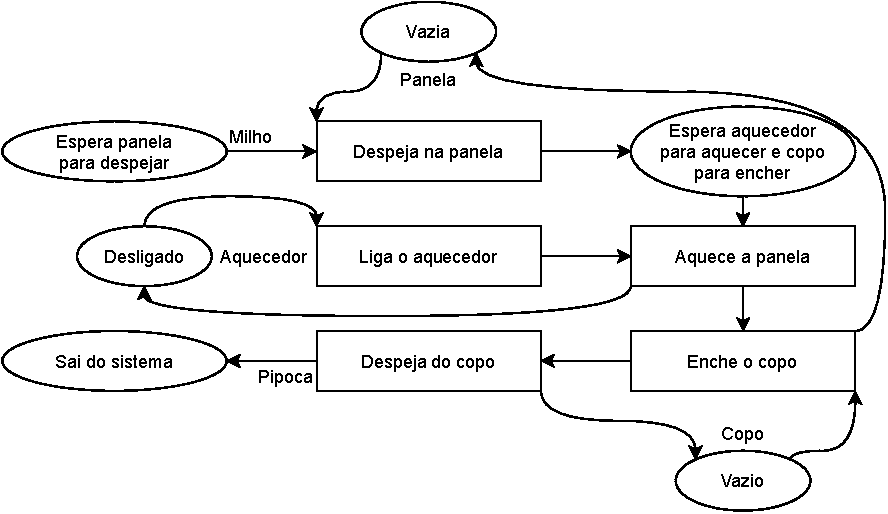
\includegraphics[width=\textwidth]{figuras/acd}
    \caption{Diagrama de ciclo de produção de pipoca. Fonte: acervo próprio.}
    \label{fig:acd}
\end{figure}

Inicialmente, realizou-se o pré-processamento do dados, visando tratar os \textit{timestamps} encontrados e eliminar atributos irrelevantes. Após o devido pré-processamento, cinco atividades foram identificadas no processo produtivo: enchimento da panela, ligação do aquecedor, aquecimento da panela, enchimento do copo, e despejo do copo. Essas atividades são desempenhadas por três entidades: aquecedor, panela, e copo. As \textit{timestamps} foram utilizadas para coletar a duração de cada evento da linha de produção, valendo-se dos estados das entidades para delinear o começo e o fim de cada etapa. Como resultado destas identificações e coletas, construiu-se o \textit{Activity Cicle Diagram} (ACD) visto na \autoref{fig:acd}.

Uma vez coletados os tempos de cada etapa do processo produtivo, realizou-se o tratamento delas para a remoção de \textit{outliers} extremos e moderados, e o teste de \textit{Kolmogorov-Smirnov} foi aplicado como forma de tentar descobrir a distribuição dos dados coletados. Contudo, considerando que o arquivo analisado descreve apenas sete execuções do processo e que a filtragem de \textit{outliers} removeu algumas dessas observações em cada etapa, os resultados se mostraram inconclusivos. Dessa forma, optou-se por utilizar os tempos coletados na simulação. Os histogramas contidos na \autoref{fig:hist} descrevem a distribuição dos tempos de execução coletados para cada etapa do processo produtivo.

\begin{figure}[h]
    \centering
    
    \begin{subfigure}[b]{0.33\textwidth}%
         \centering
         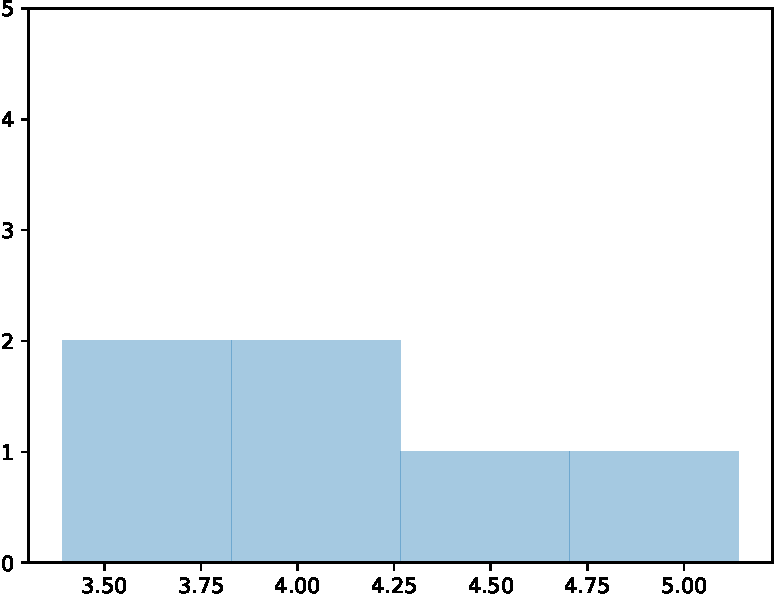
\includegraphics[width=\textwidth]{figuras/enchimento_panela}
         \caption{Enchimento da panela}
         \label{fig:hist_enchimento_panela}
     \end{subfigure}%
     \hfill
     \begin{subfigure}[b]{0.33\textwidth}%
         \centering
         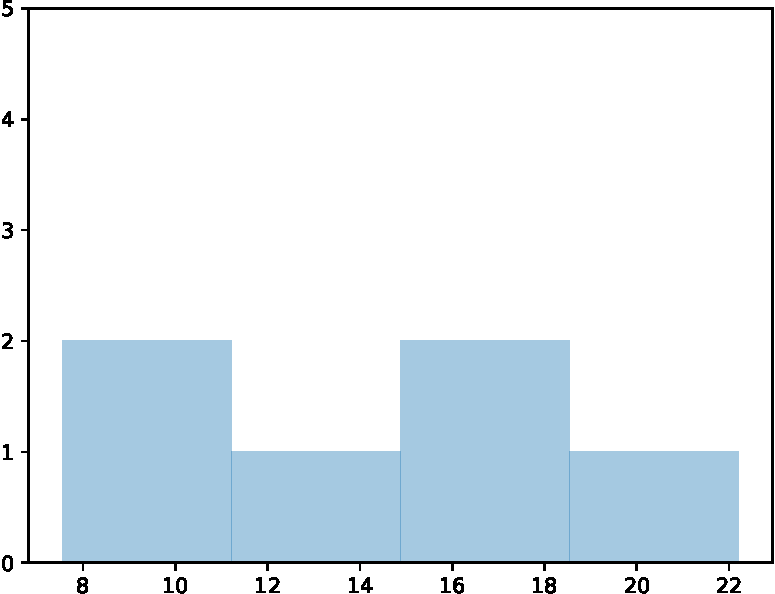
\includegraphics[width=\textwidth]{figuras/ligação_aquecedor}
         \caption{Ligação do aquecedor}
         \label{fig:hist_ligacao_aquecedor}
     \end{subfigure}%
     \hfill
     \begin{subfigure}[b]{0.33\textwidth}%
         \centering
         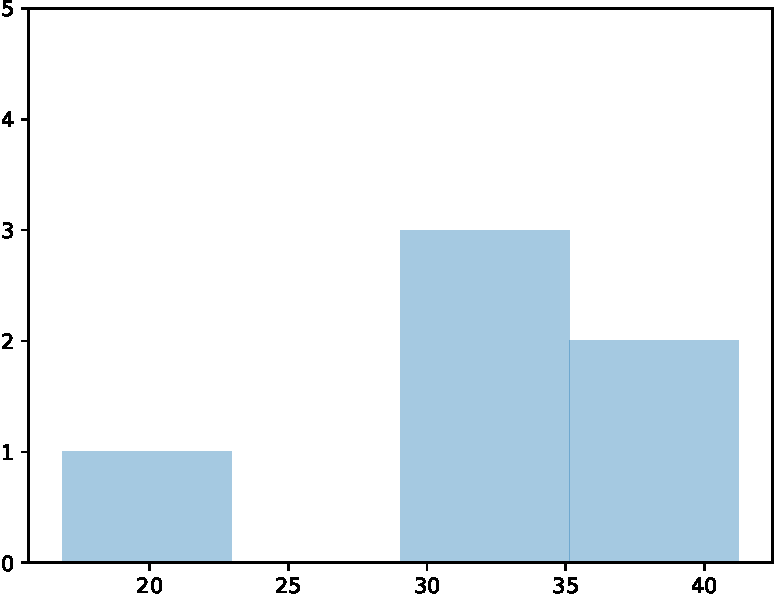
\includegraphics[width=\textwidth]{figuras/aquecimento_panela}
         \caption{Aquecimento da panela}
         \label{fig:hist_aquecimento_panela}
     \end{subfigure}%
     
     \nointerlineskip
     \vspace{4pt}
     
     \null\hfill
     \begin{subfigure}[b]{0.32\textwidth}%
         \centering
         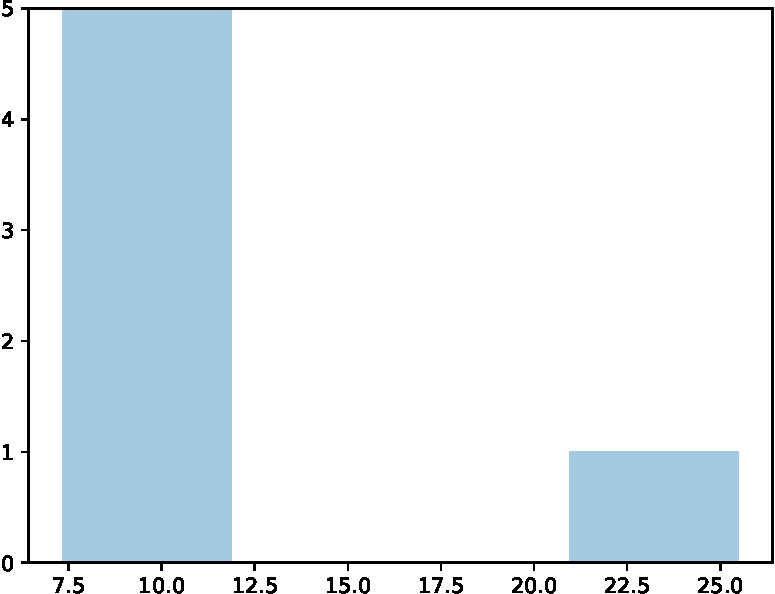
\includegraphics[width=\textwidth]{figuras/enchimento_copo}
         \caption{Enchimento do copo}
         \label{fig:hist_enchimento_copo}
     \end{subfigure}%
     \hspace{4pt}
     \begin{subfigure}[b]{0.32\textwidth}%
         \centering
         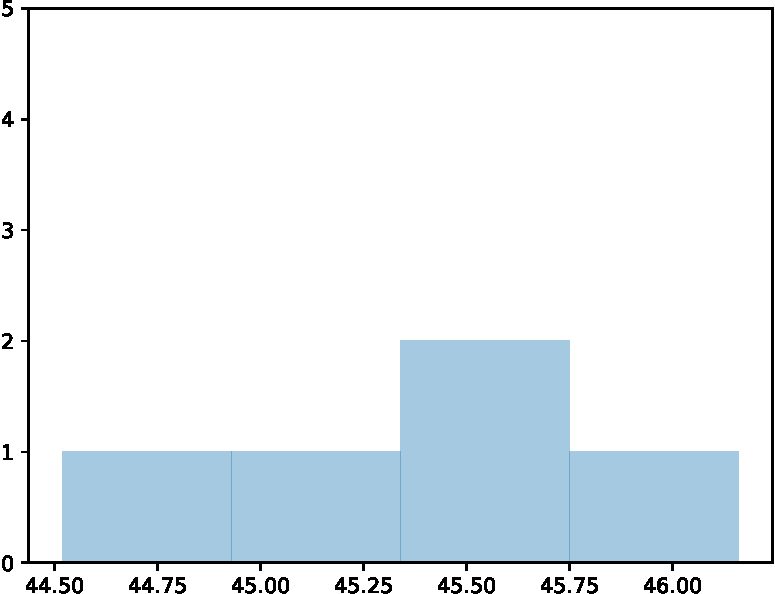
\includegraphics[width=\textwidth]{figuras/despejo_copo}
         \caption{Despejo do copo}
         \label{fig:hist_despejo_copo}
     \end{subfigure}%
     \hfill\null
    
    \caption{Distribuições dos tempos de execução de cada etapa da simulação. Fonte: acervo próprio.}
    \label{fig:hist}
\end{figure}

\section{Simulação e Resultados}
\label{sec:simulacao_resultados}

Nesta seção, as simulações realizadas tomando como base o processo obtido a partir do arquivo \texttt{Production.csv} estão descritas. A fim de facilitar as comparações entre os experimentos, um tempo limite comum de uma hora foi estipulado para todas as simulações. Todas as simulações ora descritas foram executadas mil vezes.

A primeira simulação realizada (referida doravante como simulação \textit{baseline}) buscou seguir o fluxo original obtido a partir do conjunto de dados, a fim de ter-se um desempenho contra o qual comparar os experimentos subsequentes feitos na simulação, que alteram o processo produtivo.

Após a obtenção de medidas do primeiro experimento, duas particularidades saltaram aos olhos. Em primeiro lugar, o aquecedor é constantemente desligado e ligado, o que faz com que o tempo de ligação do aquecedor seja considerado. Em segundo lugar, uma vez que há apenas uma panela, há de se considerar também o tempo de despejo do milho na panela. Com base nessas observações, dois possíveis melhoramentos foram cogitados: deixar o aquecedor sempre ligado, e adicionar uma segunda panela à simulação, tal que, enquanto uma está em uso pela máquina, a outra está sendo enchida de milho em preparação para a produção da próxima porção.

A partir das duas possíveis melhorias, três experimentos foram concebidos: dois em que apenas uma das melhorias são utilizadas em isolamento, e um terceiro em que ambas são empregadas. Os resultados deles, bem como do experimento \textit{baseline}, podem ser vistos na \autoref{fig:resultados}, a partir da qual algumas coisas podem ser depreendidas:

\begin{itemize}
    \item Deixar a panela sempre cheia, considerando os tempos de enchimento coletados a partir do conjunto de dados, gerou uma melhoria tímida no processo.
    \item Em contraste, deixar o aquecedor sempre ligado resultou em um ganho de desempenho mais significativo.
    \item Conforme o esperado, empregar ambas as melhorias resultou em um ganho ligeiramente maior em relação ao emprego apenas do aquecedor sempre ligado.
\end{itemize}

\begin{figure}[ht]
    \centering
    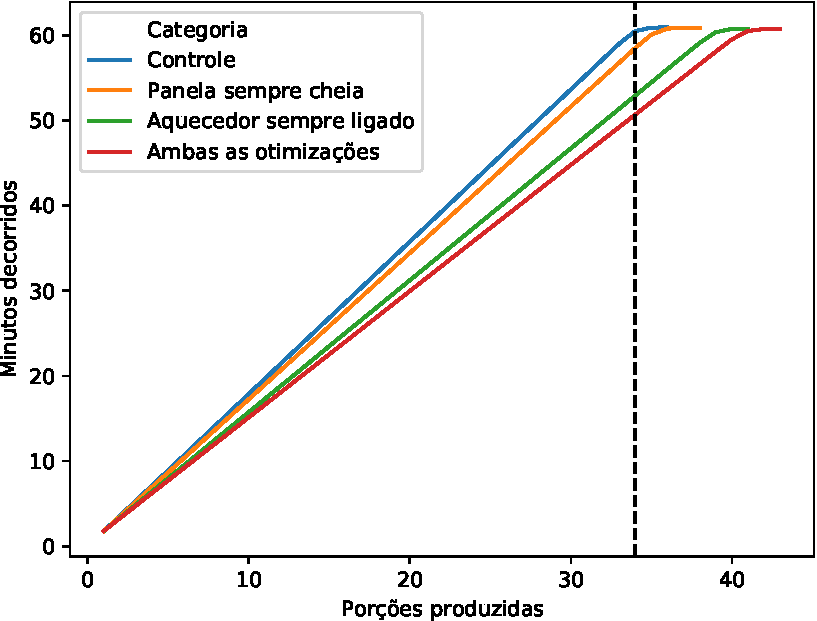
\includegraphics[width=\textwidth]{figuras/resultados}
    \caption{Resultados de simulação médios a partir de mil execuções de quatro experimentos. Fonte: acervo próprio.}
    \label{fig:resultados}
\end{figure}

\begin{table}[t]
    \centering
    \caption{Resultados de produtividade de pipoca em uma hora, estratificados por experimento. Fonte: acervo próprio.}
    \begin{tabular}{lrr}
        \toprule
        {} & \textbf{Porções produzidas} & \textbf{Tempo médio por unidade}\\
        \textbf{Categoria} & {} & {\textbf{(minutos)}}\\
        \midrule
        Controle                & 34.03 $\pm$ 0.70 & 29.50 $\pm$ 16.53\\
        Panela sempre cheia     & 35.35 $\pm$ 0.70 & 28.46 $\pm$ 15.91\\
        Aquecedor sempre ligado & 39.08 $\pm$ 0.71 & 25.79 $\pm$ 14.31\\
        Ambas as otimizações    & 40.77 $\pm$ 0.80 & 24.71 $\pm$ 13.68\\
        \bottomrule
    \end{tabular}
    \label{tab:resultados}
\end{table}

Os dados contidos na \autoref{tab:resultados} confirmam as intuições obtidas da \autoref{fig:resultados}. O mero emprego do aquecedor sempre ligado resultou em uma produtividade de porções aproximadamente 15\% maior, enquanto que a aplicação das duas otimizações aumentou esse ganho para quase 20\%.

\section{Proposta de Melhorias e Simulações}
\label{sec:propostas}

Conforme descrito na seção anterior, duas das melhorias cogitadas para o processo produtivo sob análise são: manter o aquecedor sempre ligado (eliminando o tempo de ligação do aquecedor), e ter uma segunda panela, já preenchida com milho, pronta para a produção da próxima porção (eliminando o tempo de enchimento da panela).

A \autoref{fig:resultados} e a \autoref{tab:resultados} expõem um aumento expressivo de produtividade nas simulações quando deixamos o aquecedor sempre ligado. Se combinarmos isso com a prática de manter a panela sempre cheia, conseguimos ganhos ainda maiores, embora esse segundo ganho seja mais tímido quando comparado com o primeiro. No entanto, hão de se considerar também alguns aspectos relevantes inerentes a ambas as propostas de melhoria.

Manter o aquecedor sempre ligado vem com um custo energético que deve ser compensado pela produtividade adicional. Nesse sentido, seria interessante analisar os custos de energia de forma a estimar se o ganho seriam restritos à velocidade de produção ou se também incluiriam os lucros como consequência. A depender das conclusões obtidas, um reajuste no preço unitário seria necessário, o que também haveria de ser avaliado.

Adicionar uma segunda panela ao sistema implicaria alterações no processo produtivo, cuja viabilidade prática também deve ser discutida. Como um exemplo, pode-se conjecturar que para os tempos de enchimento de panela coletados, o tempo de enchimento da panela seria substituído pelo tempo de troca de panelas (i.e., trocar-se-iam seis por meia dúzia). Contudo, pode-se contra-argumentar que, caso as quantidades das porções sejam aumentadas, o tempo de enchimento delas seria aumentado enquanto o tempo de troca das panelas permaneceria constante, maximizando os ganhos de produtividade (uma panela, nesse caso, encheria mais de um copo).

Em ambas as melhorias, há de se monitorar a qualidade da pipoca, a fim de saber se a constante emissão de calor por parte do aquecedor ou a maior quantidade de milho por porção (se pertinente) resultariam em alguma queda de qualidade da pipoca produzida.

Abordar os questionamentos e as conjecturas expostas acima requereria informação que não consta nos conjuntos de dados analisados e que, portanto, não foi considerada nas simulações (e.g., energia consumida, tempo de troca de panelas). Dessa forma, embora os resultados obtidos suscitem a crença de que ambas as propostas de melhoria são benéficas, informação adicional se faz necessária de forma a tomar uma decisão melhor embasada.

% Quanto à questão de termos uma panela permanentemente cheia no nosso sistema, entramos numa discussão um pouco mais relacionada à qualidade da pipoca. Veja, para mantermos a panela cheia precisamos estabelecer uma maneira de manter um "fluxo de pipoca" por assim dizer para evitar o acúmulo de grãos por tempo excessivo, o que pode prejudicar a qualidade do produto final.

\section{Conclusão}
\label{sec:conclusao}

Neste artigo, um processo produtivo de produção de pipoca foi analisado e simulado. Um ACD descrevendo o \textit{pipeline} da simulação do processo original foi produzido a partir do escrutínio do conjunto de dados. Após simular o processo \textit{baseline} (i.e., o processo produtivo original), dois aspectos potencialmente passíveis melhoria foram considerados: o do enchimento e o do aquecimento da panela. Ambos foram alvos de melhorias, que foram simuladas isoladamente e conjuntamente, e comparadas com a simulação \textit{baseline}.

Os resultados expuseram que ambas as melhorias são promissoras em alguma medida, tanto em termos de tempo de produção por unidade (que foi reduzido) quanto de número de porções produzidas por hora (que foi aumentado). Uma vez expostos, os resultados foram analisados e alguns questionamentos foram levantados no tocante à viabilidade e aos desdobramentos da implementação das melhorias no processo produtivo.

Como conclusão, tem-se que as melhorias propostas se mostraram auspiciosas nas simulações realizadas. Uma vez que esses ganhos são acumulados à medida em que o processo produtivo é repetido, tem-se que os ganhos de produtividade a longo prazo seriam ainda maiores, permitindo reduzir o tempo de execução da máquina e obter a mesma produção ou maximizar a produtividade mantendo o mesmo tempo de execução. Entretanto, faz-se necessária a ressalva de que, conforme abordado na seção anterior, dados adicionais seriam necessários para conferir maior confiabilidade nas análises realizadas. Não se sabe, por exemplo, se deixar o aquecedor constantemente ligado resultaria em um gasto de energia superior a quaisquer benefícios dele advindos, nem se a adição de uma segunda panela ao sistema efetivamente valeria a pena ou não. Tais análises, no entanto, estão além do escopo e do propósito deste artigo.

A quem interessar possa, a implementação da simulação em \textit{Python} está disponível na plataforma \textit{GitHub} no repositório \href{https://github.com/ygarasab/popcorn-production}{@ygarasab/popcorn-production}.

\bibliographystyle{sbc}
\bibliography{bibliografia}

\end{document}
